
\section{Using YOLOv5 assistant feature maps for matching finger knuckle}

\begin{figure}[ht!]
    \centering
    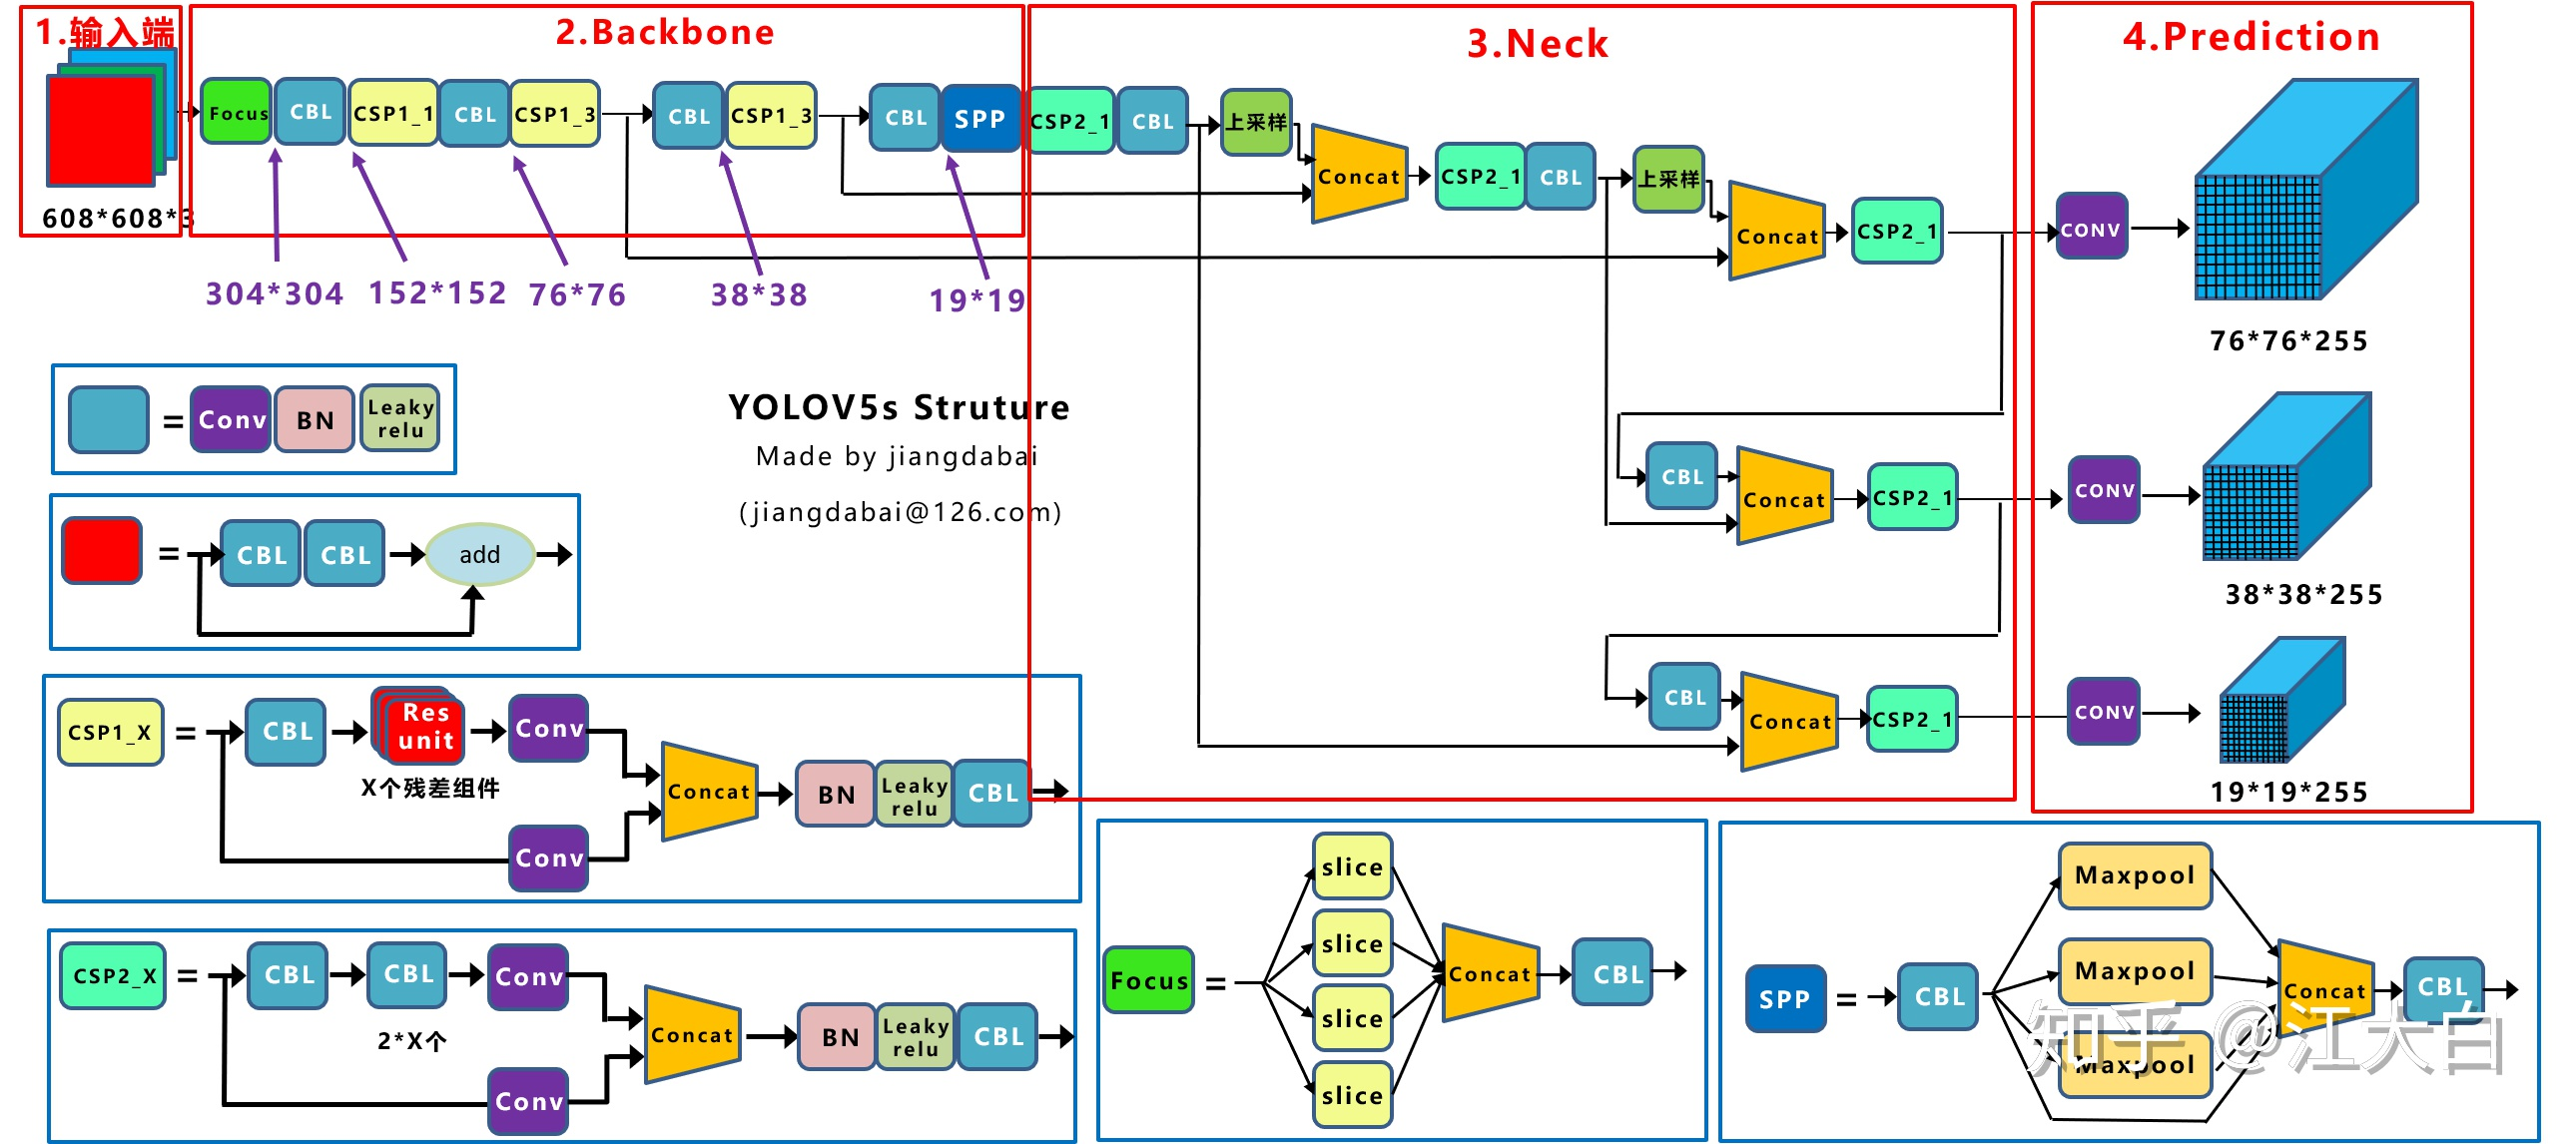
\includegraphics[width=6in]{Figure/29-10-2022/yolov5s.jpg}
    \caption{Yolov5s model structure which contains backbone, neck, and prediction part for object detecting.}
    \label{yolov5s}
\end{figure}

From the Fig. \ref{yolov5s}, the YOLOv5 model uses the backbone the extract feature maps of objects, while uses the neck part to fusion different resolution feature maps. Therefore, the backbone and neck part mainly aims to extract robust feature from input images for the prediction part to predict the bounding boxes. In this kind of situation, we have already trained the model to detect finger knuckle in the wild scenarios result in getting robust features of finger knucke. \textcolor{red}{I directly extract the feature of finger knuckle from neck part output. We can get outputs feature maps of three different sizes, 1/8 of the input image (Stride 8), 1/16 of the input image (Stride 16), and 1/32 of the input image (Stride 32) from the neck part.}

\subsection{Locate the position of finger knuckle in the feature map}
We can get the finger knuckle bounding boxes from the prediction output, but the position and size is based on the size of input images. If we want to get the feature of finger knuckle on the YOLOv5's feature maps, we should reduce the bounding boxes size based on the feature maps size. With the predicted bounding boxes information, we can rotate features maps and crop the finger knuckle features from the entire image feature maps. 

\subsection{Matching finger knuckle directly using feature maps from YOLOv5}

After cropping finger knuckle features from the YOLOv5, we can get 3 different size features because the YOLOv5 have 3 different size feature maps of neck part. \textcolor{red}{One key point is how to use these features to matching finger knuckle.} And different finger knuckle has different size on the input images results in different size of the feature maps of finger knuckle. The height and width are different, but the channels of feature maps always keep the same size. \textcolor{red}{For examples, the Stride 8 finger knuckle feature size is $h\times w \times 1280$. For keeping the same feature size, I get the maximal value of each channel, so the size will become $1 \times 1280$}. Therefore we get $1 \times 640$ feature vector from Stride 16, and get $1 \times 1280$ feature vector from Stride 32

\subsubsection{ROC curve results by using located feature}

\begin{figure}[h]
    \centering
    \subfloat[]{
        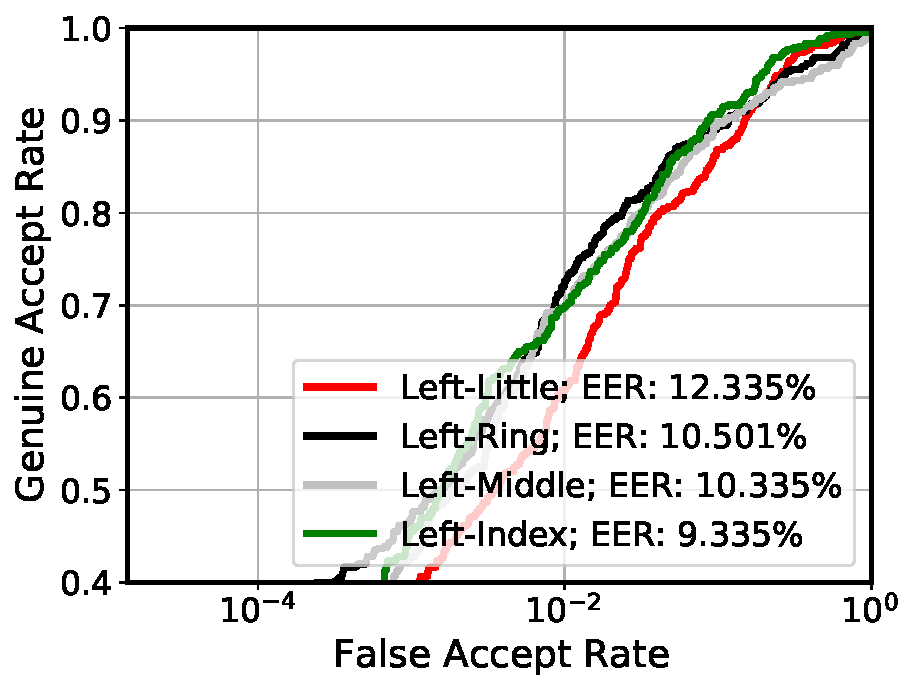
\includegraphics[width=2.8in]{Figure/29-10-2022/stride8-roc.pdf}
        \label{}}
    \subfloat[]{
        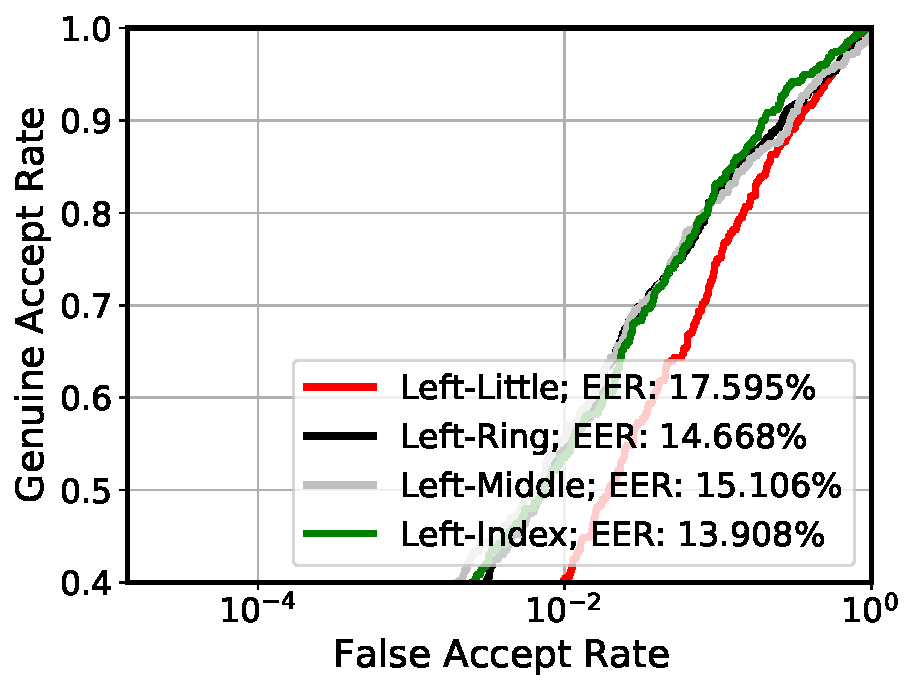
\includegraphics[width=2.8in]{Figure/29-10-2022/stride16-roc.pdf}
        \label{}}

    \subfloat[]{
        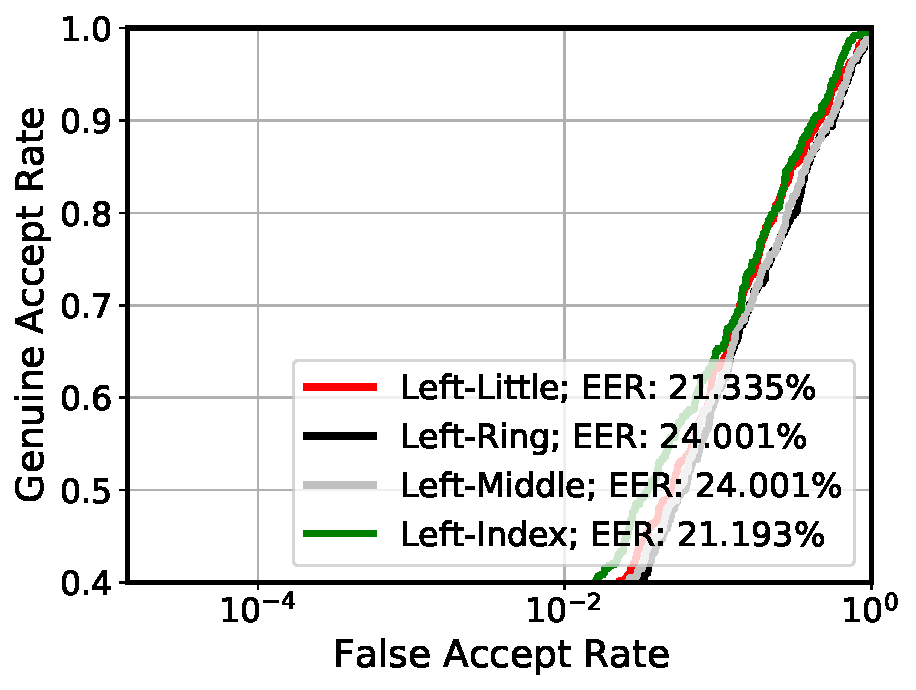
\includegraphics[width=2.8in]{Figure/29-10-2022/stride32-roc.pdf}
        \label{}}
    \subfloat[]{
        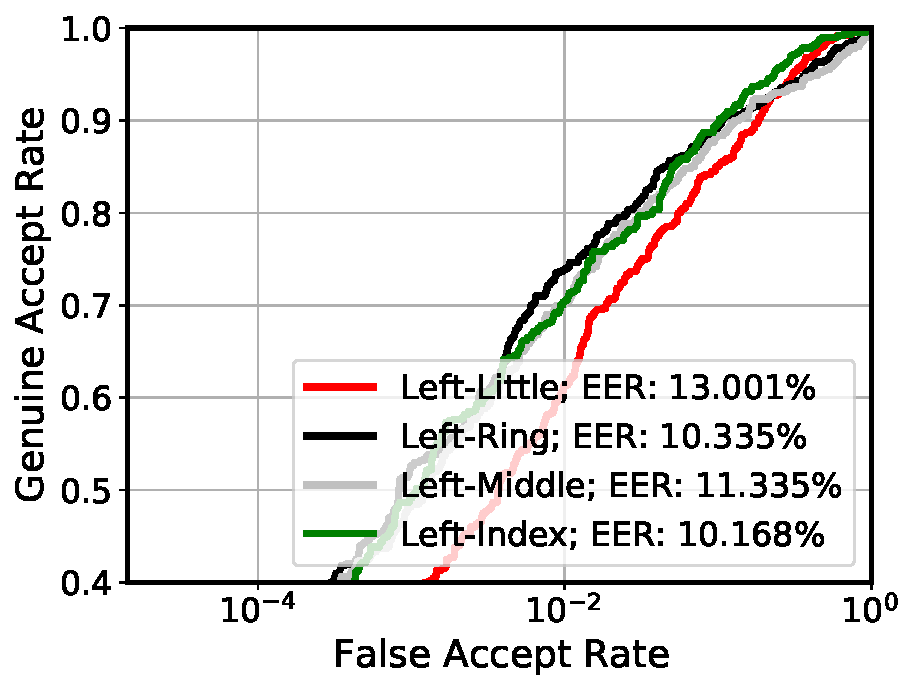
\includegraphics[width=2.8in]{Figure/29-10-2022/stride8-stride16-stride32-roc.pdf}
        \label{}}

    \caption{Matching performance with (a) only use Stride 8 feature, (b) only use Stride 16 feature, (c) only use Stride 32 feature, and (d) use all of them}
    \label{roc}
\end{figure}
From the Fig. \ref{roc}, we can get the conclusion that the Stride 8 has more robust features than the Stride 16 and Stride 32. Because its field of view is smaller than the rest, and more focus on the finger knuckle. The Stride 8 and Stride 32 have bigger field of view result in getting more background information (semantic information) that is not useful for matching finger knuckle.

\subsection{Plans}
\begin{itemize}
    \item Fusing the features from the YOLOv5 and the features from the segmented finger knuckle
    \item Fusing the finger knuckle and fingerprint
    \item Comparing the performance of EfficientNet and DoN model
\end{itemize}





